
\section{Type classes}
\label{sec:typeclasses}

This section will give a short description of the concept type class. It will explain the relation to polymorphism and describe type classes \verb|Functor|, \verb|Applicative| and \verb|Monoid| in more detail as these type classes are important for the example in section \ref{sec:example}.

The concept of a type class was introduced as a construct that supports operator overloading and ad-hoc polymorphism \cite{Wadler}.

A type classes are often compared to interfaces. It contains the function declarations. A type becomes an instance of a type class when it defines all required functions of the type class. When a type is an instance of a type class, we can make certain assumptions about behavior of the type. In contrary to interfaces, type classes aren't types. A value can have the type of an interface but not of a type class. Another difference to interfaces is that type classes describe functions and the instance types are part of the function signature. The instance type can be the return type. Interfaces define methods of the instance type.

The concept of a type class is explained by example with the function \verb|show| from the \verb|Prelude|-Library (\verb|Prelude| is a module and part of the standard). \verb|show| converts a given value of a type \verb|a| into a character string. The type of \verb|show| is

\begin{verbatim}
show :: Show a => a -> String
\end{verbatim}

The \verb|Show a| before the \verb|=>| is a type class constraint. \verb|a| is a type variable. A type that has one more type variables is called polymorphic \cite{hutton}. The signature means that \verb|show| takes something that implements the type class \verb|Show| and returns a string. \verb|Show| is a type class. It's possible to call \verb|show| with different types (e.g \verb|show 1|, \verb|show "hello"|). The compiler will look up the correct definition for us as long the type of the first parameter is an instance of the type class \verb|Show|.  
Any type that implements \verb|Show| can be converted to a character string. Types in this class are \verb|Bool|, \verb|Char|, \verb|Int|, \verb|Float|, \verb|Double| etc.

The type class \verb|Show| is defined as follows:
\begin{verbatim}
class Show a where
    show :: a -> String
\end{verbatim}
The keyword \verb|class| defines a new type class. \verb|a| is the type variable. It represents the type that implements the type class (e.g. \verb|Int| or \verb|Bool|).

Once we have a type class we are able to create instances of that class. The following listing defines a type \verb|Person|. It has fields for name and email address. 
\begin{verbatim}
data Person = Person { name :: String
                       email :: String
                     }
\end{verbatim}

To make \verb|Person| an instance of \verb|Show| we provide a function with the following type:
\begin{verbatim}
show :: Person -> String|
\end{verbatim}

\begin{verbatim}
instance Show Person where
    show (Person name _) = name
\end{verbatim}

There many other useful type classes in the standard library.

\begin{description}
\item[Ord] Types with an order relation implement \verb|Ord|.
\item[Eq] For types that can be equated.
\item[Read] Types that can be converted from a string.
\end{description}

\subsection{Polymorphism and type classes}
\label{sec:polymorphism}
In this section we will describe relation between type classes and polymorphism.
There are two types of polymorphism in Haskell \cite{Cardelli}. Type classes are used for ad hoc polymorphism.
\begin{description}
\item[Parametric polymorphism] Refers to a type that contains type variables. For example the type of the function \verb|id| is 
\begin{verbatim}
id:: a -> a
\end{verbatim}
The \verb|id| function can be used with any type. There are no constraints. At compile time, the type variables are substituted with a concrete type. For example
\verb|Char -> Char|.
\item[Ad-hoc polymorphism] It's a synonym for function overloading or operator overloading. Polymorphic functions can be applied to values with different types. A polymorphic function uses different definitions (implementations) depending on the types of the arguments. If a type can be converted to a string, it can be given the type class \verb|Show|. The type \verb|Person| has to provide an implementation for the function \verb|show|. Applying \verb|show| to \verb|Person| results in a different behavior then applying \verb|show| to an \verb|Int|.
\end{description}

\subsection{Functor}
\label{sec:functor}

Functor is a type class for types, which can be mapped over. Another way to describe functors is, that they represent some sort of computational context \cite{yorgey}. The general concept of a functor is more abstract and harder to grasp than the concepts of type classes described above \footnote{this is personal impression}.
The most accurate way to describe the type class \verb|Functor| is to give it's declaration \cite{data.functor}:

\begin{verbatim}
class Functor f where
    fmap :: (a -> b) -> f a -> f b
\end{verbatim}

The \verb|f| in the declaration is a type class constructor. Only type constructor can implement \verb|Functor| (\verb|Maybe|, \verb|[]|).

\verb|fmap| takes any function \verb|a -> b| and a value of type \verb|f a| (\verb|f| is the container or context, \verb|a| is the type wrapped inside the functor) and returns a value of type \verb|f b|. 
If \verb|f a| is of type \verb|Maybe| \verb|Int| and the function of type \verb|Int -> String|, \verb|fmap| returns \verb|Maybe String|. 

Instances of \verb|Functor| are:

\begin{description}
\item[List] \verb|map| for lists for is the same as \verb|fmap|.
\item[Either] \verb|Either e a| is a container. \verb|fmap| applies a function to \verb|a|.
\end{description}

To make a type an instance of \verb|Functor|, it has to define \verb|fmap|. In addition the instances of are expected to exhibit certain kinds of properties. The declaration of the type class doesn't reveal this properties. There are described in the type class documentation \cite{data.functor} \cite{Marlow_2010}. This properties are called the functor laws.
The Haskell Compiler doesn't detect violations of the expected laws. All Functor instances in the standard library obey these laws \cite{yorgey} \cite{Lipovaca}.

A Functor instance has to satisfy the following laws.

\begin{description}
\item[Law 1] Mapping the identity function over a functor value, will not change the functor value. Formally
\begin{verbatim}
fmap id  ==  id
\end{verbatim}
\item[Law 2] It doesn't matter if we compose two functions and them map them over a functor or if we first map one function over the functor and then map the other function. Formally
\begin{verbatim}
fmap (g . h) = fmap g . fmap h
\end{verbatim}
This is the same as \verb|fmap (g . h) = fmap g (fmap h)|
\end{description}

If we can prove that a type satisfies these laws, we can make assumptions about how the the type will act. We know that \verb|fmap| will not change the structure or the context of the functor.
And we know that \verb|fmap| only maps the function over the functor and nothing else. 

If we know, that a type satisfy the laws, we are able to deduce further properties for our own types. In section \ref{sec:example} give an example of this process.

\begin{figure}
  \centering
\begin{verbatim}
fmap id = id
fmap (g . h) = fmap g . fmap h
\end{verbatim}
  \caption{The Functor laws}
  \label{fig:functorlaws}
\end{figure}

\subsection{Applicative Functor}
\label{sec:applicatives}

Applicative functors are an abstract characterization of an applicative style of effectful programming \cite{mcbride} \cite{control.applicative}

The \verb|Applicative| type class encapsulates the following idea. What if you have a function wrapped in a \verb|Functor| (e.g. \verb|Maybe (Int -> Int -> Int)|) and you want to apply the function to another functor (e.g. \verb|Maybe Int|). For example we want to map \verb|Just (3 *)|, a function encapsulated inside a functor, over \verb|Just 23|, another functor with an encapsulated \verb|Int|? \verb|fmap| doesn't work here, because it expects a normal function \verb|a -> b| as first parameter. That's where the \verb|Applicative| type class come in. 
The \verb|Applicative| type class is defined as follows \cite{control.applicative}.
\begin{verbatim}
class (Functor f) => Applicative f where
    pure :: a -> f a
    (<*>) :: f (a -> b) -> f a -> f b
\end{verbatim}

The type class declaration demands the type \verb|f| to be a functor. Every type that is part of \verb|Applicative| is part of \verb|Functor|. Hence we can use \verb|fmap| with \verb|Applicative| instances.
Applicatives are enhanced functors. In addition to to \verb|fmap| we can use the \verb|<*>| operator to chain several applicative values together.

The \verb|pure| function puts a value of type \verb|a| in a default context. If applied with a function \verb|a -> b| pure return a functor with a function inside, hence the first argument to \verb|<*>|.

It possible to chain applicative together as follows:
\begin{verbatim}
ghci> pure (*) <*> Just 3 <*> Just 23
Just 69
\end{verbatim}

The following type are instances of the type class \verb|Applicative|

\begin{itemize}
\item Maybe
\item Lists
\item IO
\end{itemize}

There are several laws that \verb|Applicative| instances should satisfy \cite{mcbride} \cite{control.applicative}. This article will describe only the following, as it defines the relation to the \verb|Functor| type class.

\begin{verbatim}
fmap g x = pure g <*> x
\end{verbatim}

The law says that applying \verb|fmap| over a normal function \verb|g| over a functor \verb|x| is the same as putting \verb|g| in a default context and mapping the resulting function over \verb|x|. Figure \ref{fig:functor_applicative} illustrates the relation between \verb|Functor| and \verb|Applicative|.

\begin{figure}
  \centering
     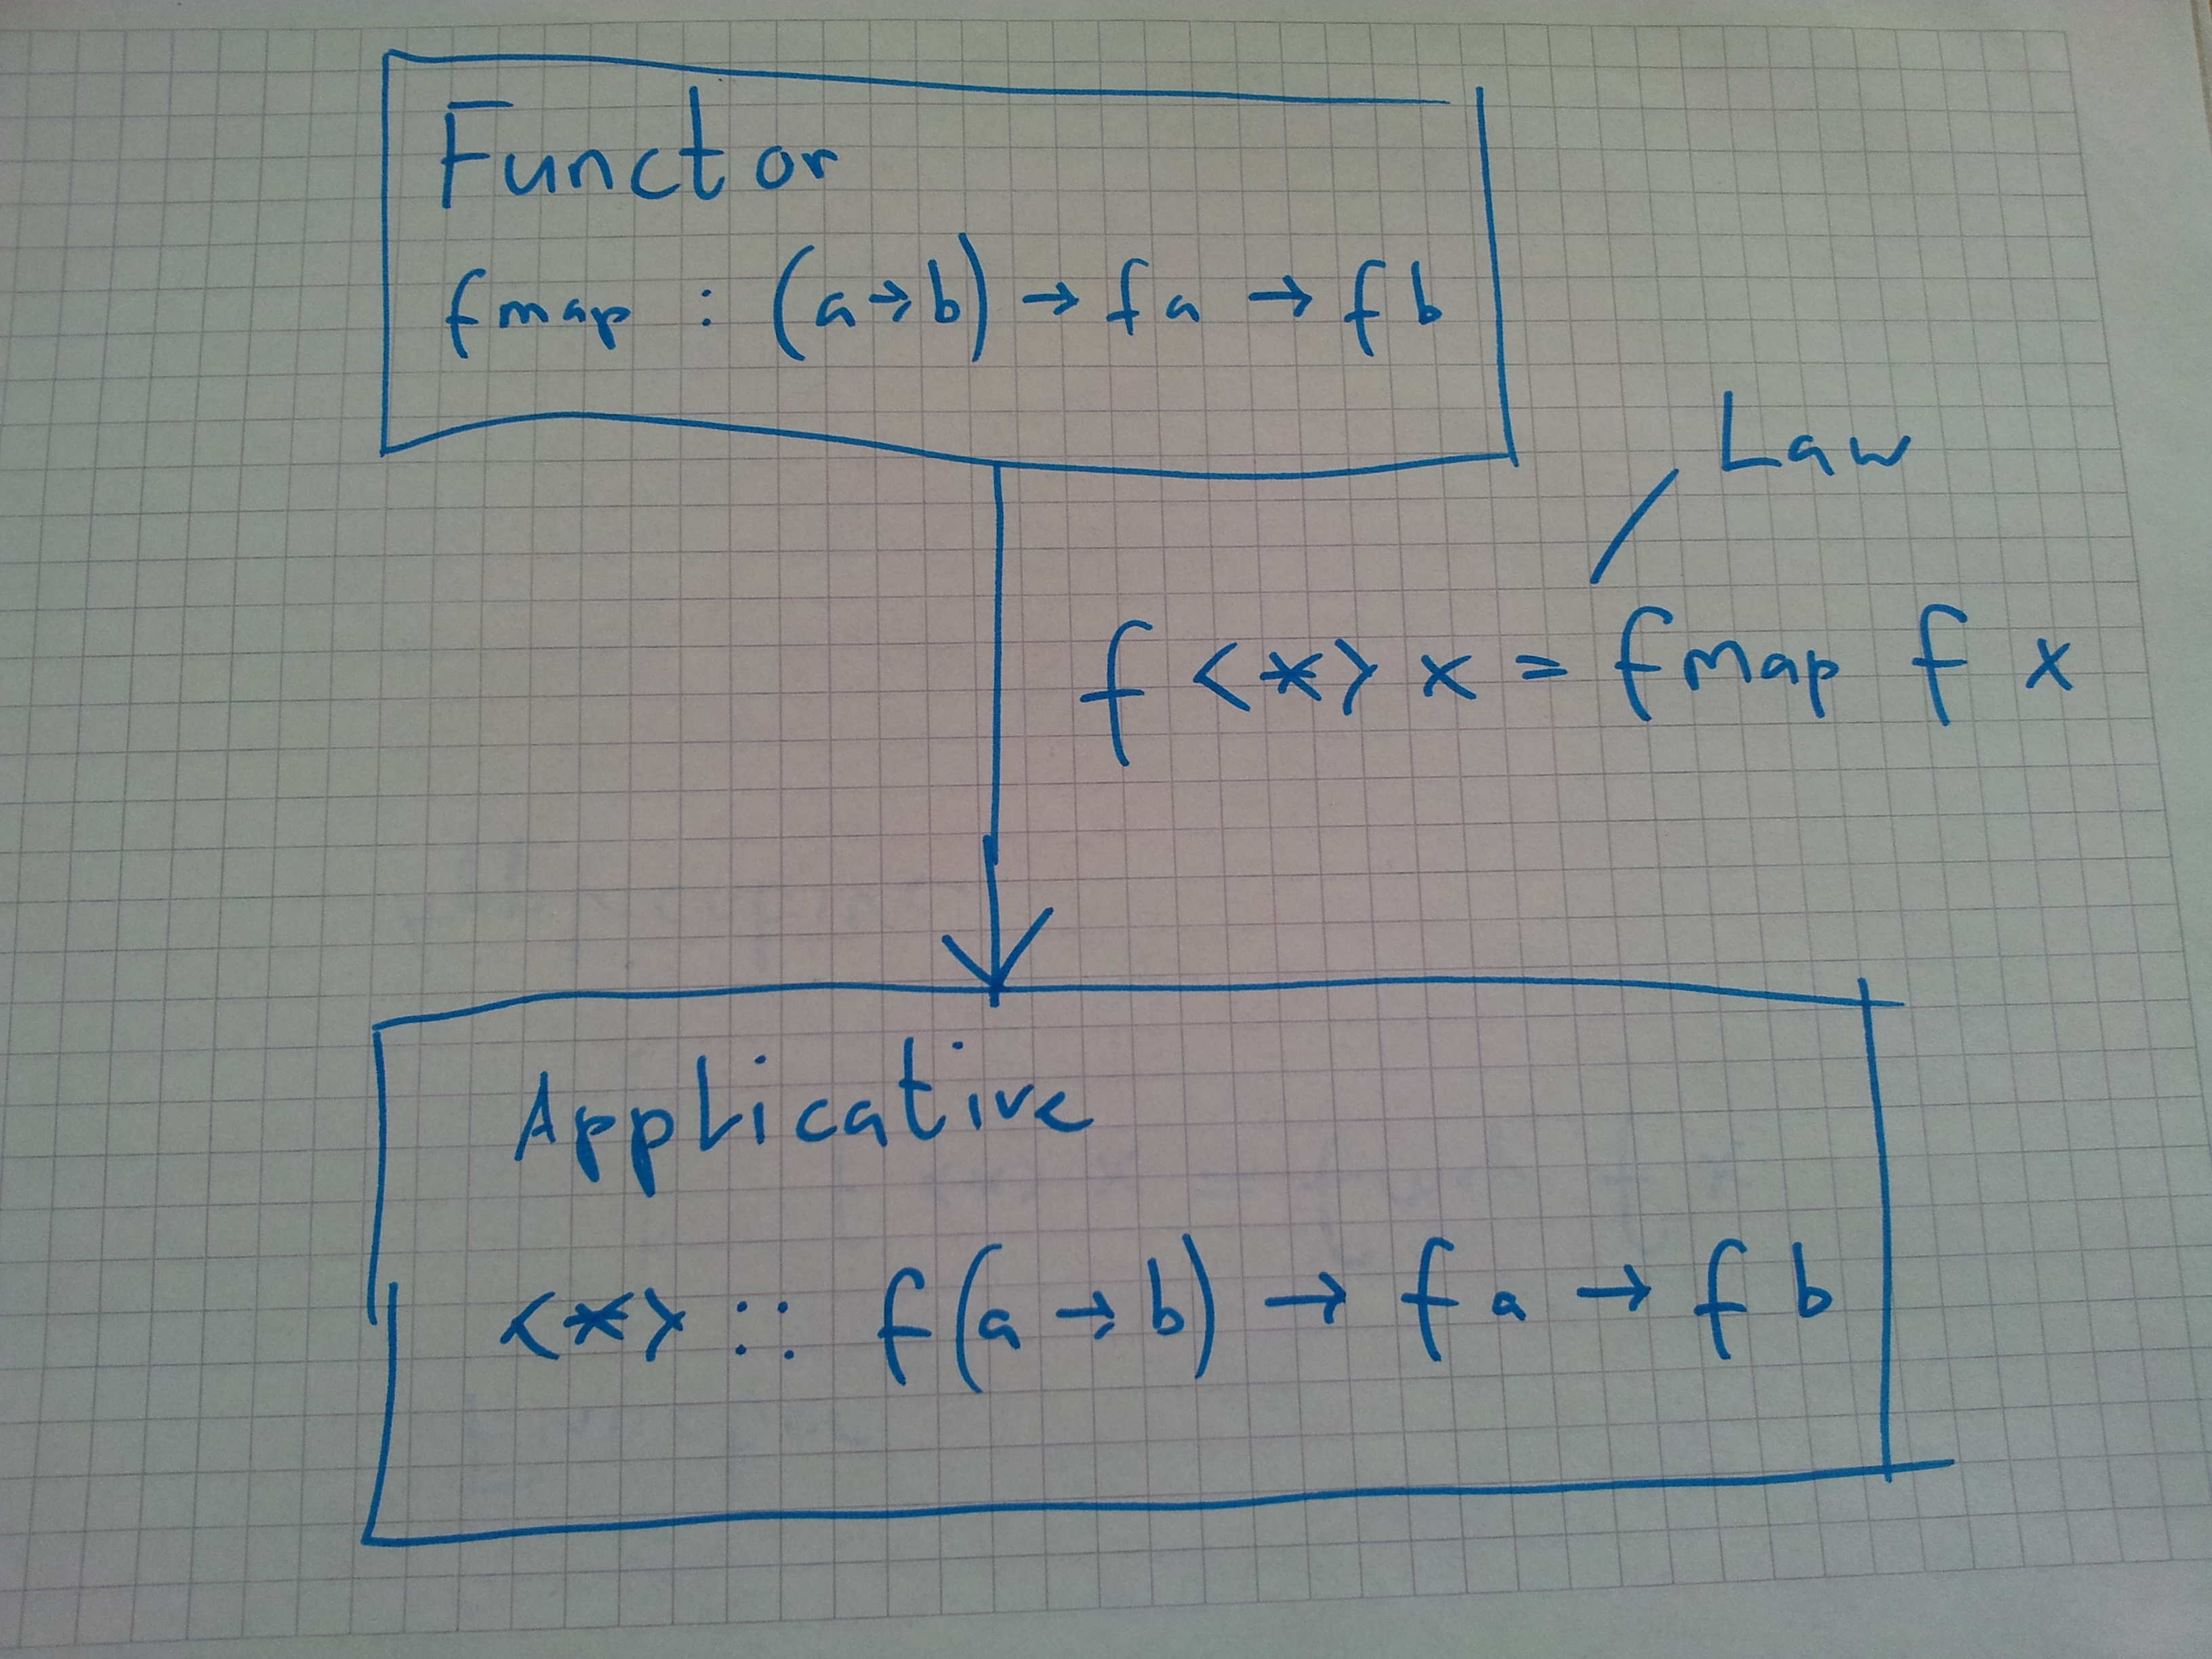
\includegraphics[width=0.9\textwidth]{functor_applicative}
  \caption{Interrelationship of Functor and Applicative}
  \label{fig:functor_applicative}
\end{figure}

\subsection{Monoid}
\label{sec:monoid}

Monoids contain types with the following behavior. 
Some types, let's say \verb|a|, have a binary function with the type declaration. 
\begin{verbatim}
f :: a -> a -> a
\end{verbatim}

The type \verb|a| has a value that serves as identity for the given function. For example the number 1 is the identity for the multiplication. Multiplication of the identity and any other number $x$ results always in $x$.

Several value of type \verb|a| can always be reduces to a single value. It doesn't matter in which order we apply the function, the result is always the same. This is called associativity.

If type \verb|a| has this behavior, it's a monoid and it can be an instance of the \verb|Monoid| type class.

The \verb|Monoid| type class is define as follows \cite{monoid}:
\begin{verbatim}
class Monoid m where
    mempty :: m
    mappend :: m -> m -> m
    mconcat :: [m] -> m
    mconcat = foldr mappend mempty
\end{verbatim}

The \verb|Monoid| type class is define in \verb|Data.Monoid|. 

From the type class declaration we see that concrete types can be part of the \verb|Monoid| type class. 

\verb|mempty| returns the identity value. The binary function is \verb|mappend|. It takes to values of the same type and returns another value of that type. \verb|mconcat| takes a list of monoids and reduces them \verb|mappend| to a single value, applying mappend. It has a default implementation.

The following Haskell types are \verb|Monoid| instances
\begin{description}
\item[List] The empty list \verb|[]| and \verb|++| (concatenation) form a monoid.
\item[Product and Sum] Numbers can be monoid with respect to multiplication or addition. There are two monoid instances for \verb|Num|.
\item[Maybe] Can also be an instance of \verb|Monoid|.
\end{description}

When making monoid instances, we need to make sure that \verb|mempty| acts like the identity with respect to the \verb|mappend| function and \verb|mappend| must be associative. There are three monoid laws \cite{monoid}.

\begin{enumerate}
\item \verb|mappend mempty x = x|
\item \verb|mappend x mempty = x|
\item \verb|(x `mappend y) `mappend z = x `mappend (y `mappend z)|
\end{enumerate}

There is a useful property of the \verb|Applicative| type class with respect to the \verb|Monoid| type class: If \verb|f| is an \verb|Applicative| and \verb|m| is a \verb|Monoid|, \verb|f b| is also a \verb|Monoid|. If a type is part of the \verb|Applicative| we can create a \verb|Monoid| instance with the implementation in listing \ref{lst:applicative2monoid}.

\begin{program}
\begin{verbatim}
instance (Applicative f, Monoid b) => Monoid (f b) where
    mempty = pure mempty

    mappend = liftA2 mappend
\end{verbatim}
\label{lst:applicative2monoid}
\caption{Applicative property}
\end{program}

As \verb|f| is an applicative, it implements \verb|pure|. The \verb|mempty| function returns the identity value of \verb|b| in a default context. \verb|liftA2| is an utility function of \verb|Applicative|. It encapsulates the \verb|mappend| function in an applicative functor. 

In section \ref{sec:example} we prove this property with equational reasoning and we use it to show that a type is part of \verb|Monoid|.
